\chapter{Governing equations} \label{chap:equations} %mathematical model?
In this chapter we present the equations that we have used to model the 
free-flow and the porous-medium flow. For the free-flow we start 
considering the incompressible Navier-Stokes equations to simulate laminar 
flows, then we move to the Reynolds Averaged Navier-Stokes (RANS) equations with the $k\text{-}\omega$ 
model as a turbulence model. For the porous-medium 
flow our choice is the Forchheimer's law, which is an extension of the more 
common Darcy's law to higher Reynolds numbers.
\section{Free-flow}
\subsection{Navier-Stokes equations}
The Navier-Stokes equations describe the motion of a Newtonian viscous fluid,
defining a relation between the following physical quantities:
\begin{itemize}
	\item $\varrho$, the density of the fluid  [$\si{kg/m^3}$],
	\item $\mathbf{v} = [u, v, w]^\mathrm{T}$, the velocity vector [$\si{m/s}$],
	\item $e$, the specific total energy [$\si{J/kg}$].
\end{itemize}
They can be derived starting from the general principles of conservation of 
mass:
\begin{equation} \label{eq:masscons}
\frac{d}{dt} \int_V \varrho \; dV = 0,
\end{equation}
the second Newton's law:
\begin{equation} \label{eq:2newton}
\frac{d}{dt} \int_V \varrho \mathbf{v} \; dV = \int_V \varrho \mathbf{b} \; dV 
+ 
\int_{\partial V} \sigma \mathbf{n} \; dA
\end{equation}
and the first law of thermodynamics:
\begin{equation} \label{eq:firstthermo}
\frac{d}{dt} \int_V e \; dV = \dot{Q} + \dot{W}
\end{equation}
for any material volume $V$. In equation \eqref{eq:2newton} vector 
$\mathbf{b}$ represents possible external volume forces per unit of mass, for 
example the gravity $\mathbf{g}$, $\sigma$ is the Cauchy stress tensor 
and 
$\mathbf{n}$ is the outward unit vector normal to the surface $\partial V$ of 
$V$. In equation \eqref{eq:firstthermo} $\dot{Q}$ is the net rate of 
heat added to the fluid and $\dot{W}$ is the net rate of work done on the fluid.

For viscous fluids we can identify two contributions in the Cauchy stress 
tensor:
\begin{equation}
\sigma = -p\mathbb{1} + \tau,
\end{equation}
$-p\mathbb{1}$ is a contribution due to pressure, while $\tau$ is 
the viscous stress tensor, for which the constitutive relation of Newtonian 
fluids is used:
\begin{equation}
\tau = 2\mu \mathbf{S} + 
\lambda (\nabla \cdot \mathbf{v}) \mathbb{1},
\end{equation}
where $\mu$ is the dynamic viscosity [$\si{\pascal\second}$], $\lambda$ 
is a dilatation factor and $\mathbf{S}$ is the symmetric strain rate tensor:
\begin{equation*}
\mathbf{S} = \frac{\nabla \mathbf{v} + \nabla \mathbf{v}^\mathrm{T}}{2}.
\end{equation*} 
Moreover we define the kinematic viscosity 
[$\si{m^2/s}$] as
\begin{equation}
\nu = \frac{\mu}{\varrho}.
\end{equation}

We want to deal with incompressible fluids with a constant density that is not 
related to the pressure through a state equation. Thus, the 
energy equation can be decoupled from the others and we can exclude it from 
the system. 
Notice that, with this assumption, $p$ is no longer the thermodynamic pressure.
Using these assumptions from the balance equations 
\eqref{eq:masscons} and \eqref{eq:2newton} we obtain the incompressible Navier-Stokes 
equations:
\begin{align}
\label{eq:nsmass} \nabla \cdot \mathbf{v} = 0&\\
\label{eq:nsmom} \frac{\partial \mathbf{v}}{\partial t} + \nabla 
\cdot (\mathbf{v} \mathbf{v}^\mathrm{T}) - \nabla \cdot (\nu \nabla 
\mathbf{v}) + \frac{1}{\varrho}\nabla p  -\mathbf{g} = \mathbf{0}&
\end{align}
All the computations needed to obtain these equations can be found in any book 
of fluid mechanics, for example in \cite{main:vermal}. The continuity equation 
reduces to an incompressibility constraint \eqref{eq:nsmass} that is enforced 
in the momentum equation through the pressure that acts as a Lagrangian 
multiplier. The second term of the momentum equation \eqref{eq:nsmom} is 
non-linear and represents the advection that the velocity enforces on itself, 
while the third one is a diffusive term that express the action of the 
viscosity.
%
\subsubsection{Boundary conditions}
When the equations \eqref{eq:nsmass} and \eqref{eq:nsmom} are solved in a 
bounded domain $\Omega_\text{ff}$, suitable conditions have to be provided at 
the boundary $\partial \Omega_\text{ff}$, depending on the situation that we 
want to model. Common choices, adopted also in the test cases in Chapter~\ref{chap:results}, are the following:
\begin{itemize}
	\item on inflow boundaries, Dirichlet conditions are imposed to the 
	velocity:
	\begin{equation} \label{eq:inflow}
		\mathbf{v} = \mathbf{v}_\text{in},
	\end{equation}
	\item on solid walls, homogeneous Dirichlet conditions are imposed to the 
	velocity (also called no-slip conditions):
	\begin{equation} \label{eq:noslip}
		\mathbf{v} = \mathbf{0},
	\end{equation}
	\item on outflow boundaries, natural boundary conditions are imposed, 
	resulting in the following prescription for the stress :
	\begin{equation}
		\sigma \mathbf{n} = -p\mathbf{n}+2\mu \mathbf{Sn} = \varrho\mathbf{d},
	\end{equation}
	where $\mathbf{n}$ is the outward unit vector normal to the surface. 
	However outflow boundary conditions are usually located where the flow is 
	almost unidirectional and the surface stresses are known, so, especially 
	when using the finite volumes method, they are replaced by:
	\begin{equation} \label{eq:outflow}
	(\nabla \mathbf{v})\mathbf{n} = \mathbf{0}, \quad p = p_\text{ext},
	\end{equation}
	thus fixing a a zero-gradient condition for the velocity and imposing a 
	Dirichlet condition to the pressure (see \cite{main:vermal}).
\end{itemize}
Moreover it is usually useful to take advantage of symmetries in the flow 
field, 
when they are known because of the domain and of the boundary conditions. 
For example, to model a flow in a channel, we can impose the following 
symmetry conditions along the centre of the domain and consider only half of it:
\begin{equation}
\nabla p \cdot \mathbf{n} = 0, \quad \nabla v_t \cdot \mathbf{n} = 0, \quad
v_n = 0,
\end{equation}
where $v_t$ an $v_n$ are the tangential and normal components of the velocity.
%
\subsubsection{Reynolds number}
If we consider the non-dimensional form of equation \eqref{eq:nsmom}, scaling 
the lengths by a reference quantity $L$ and the velocities by a reference 
quantity $U$, and neglecting gravity, we obtain
\begin{equation} \label{eq:momnondim}
	\frac{\partial{\tilde{\mathbf{v}}}}{\partial \tilde{t}} + \tilde{\nabla} 
	\cdot (\tilde{\mathbf{v}} \tilde{\mathbf{v}}^\mathrm{T}) - \tilde{\nabla} 
	\cdot \bigg(\frac{1}{Re} \tilde{\nabla} \tilde{\mathbf{v}}\bigg) + 
	\tilde{\nabla} 
	\tilde{p} = 0,
\end{equation}
where $\tilde{\cdot}$ denotes non-dimensional quantities. The non-dimensional number $Re$ that multiplies the viscous term is the 
Reynolds number and it is defined as:
\begin{equation}
Re = \frac{UL}{\nu}.
\end{equation}
This quantity plays an important role characterising the behaviour of the solution of the 
Navier-Stokes equations, since it expresses the ratio between the inertial forces 
and the viscous forces. This can be easily seen in equation 
\eqref{eq:momnondim} since, when $Re\gg 1$, the viscous term loses 
importance with respect to the advective one and vice versa.

If $Re < 1$ we have a creeping flow and generally the advection term can 
be neglected, reducing the Navier-Stokes equations to the Stokes equations, 
that are much simpler to analyse and to solve because they are linear. The 
assumption of creeping flow is common in porous-media models, as we will 
see in Section~\ref{sec:pm}. If $Re>1$ we have a laminar flow, which is 
characterized by a well-ordered viscosity-dominated motion, with adjacent 
layers of the fluid that slide with little interaction between each others.
There exists a critical value $Re_c$ such that when $Re>Re_c$ a 
transition from a laminar to a turbulent flow regime starts to take place, but 
this threshold value is very problem dependent as it is affected by the 
geometry of the domain and by the boundary conditions imposed.
%
\subsection{Turbulence and RANS equations}
Turbulence is characterized by an irregular, chaotic and intermittent 
behaviour, that shows space and time fluctuations of the physical quantities 
related to the flow, as we can see in Figure~\ref{fig:fluctuations}. Due to 
this complexity, turbulence is usually studied with 
a statistical approach, relying on the theory developed by Kolmogorov 
in 1941 \cite{turbo:kolmogorov}. A complete description of turbulence can be 
found for example in \cite{main:pope}, \cite{main:wilcox} or 
\cite{main:davidson}.
\begin{figure}[ht]
	\centering
	% This file was created by matlab2tikz.
%
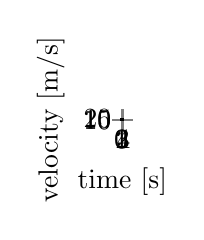
\begin{tikzpicture}

\begin{axis}[%
width=0.951\widthsette,
height=0.75\widthsette,
at={(0\widthsette,0\widthsette)},
scale only axis,
xmin=0.0003,
xmax=4.0023,
xlabel={time [s]},
ymin=10,
ymax=22,
ylabel={velocity [m/s]},
axis background/.style={fill=white},
xmajorgrids,
ymajorgrids
]
\addplot [color=black, forget plot]
  table[row sep=crcr]{%
0.0003	15.86\\
0.0063	14.5779\\
0.0123	13.6604\\
0.0183	12.8875\\
0.0243	12.4176\\
0.0303	12.6551\\
0.0363	14.0939\\
0.0423	16.3555\\
0.0483	16.7261\\
0.0543	15.9008\\
0.0603	14.9808\\
0.0663	13.9689\\
0.0723	13.455\\
0.0783	13.8104\\
0.0843	14.4593\\
0.0903	14.7927\\
0.0963	14.7728\\
0.1023	14.7752\\
0.1083	14.8455\\
0.1143	14.7653\\
0.1203	14.5008\\
0.1263	13.9457\\
0.1323	13.3764\\
0.1383	13.1549\\
0.1443	13.2625\\
0.1503	13.4964\\
0.1563	13.7114\\
0.1623	13.7333\\
0.1683	13.4597\\
0.1743	12.8486\\
0.1803	12.0619\\
0.1863	11.4672\\
0.1923	11.2568\\
0.1983	11.151\\
0.2043	10.9918\\
0.2103	10.8552\\
0.2163	10.8836\\
0.2223	11.1893\\
0.2283	11.6717\\
0.2343	12.5418\\
0.2403	14.2533\\
0.2463	16.6234\\
0.2523	17.7437\\
0.2583	17.3127\\
0.2643	16.9952\\
0.2703	16.7505\\
0.2763	15.918\\
0.2823	14.8688\\
0.2883	14.2\\
0.2943	14.2536\\
0.3003	14.7781\\
0.3063	14.6915\\
0.3123	13.9757\\
0.3183	14.1038\\
0.3243	15.1628\\
0.3303	15.7353\\
0.3363	15.4467\\
0.3423	15.1117\\
0.3483	15.3946\\
0.3543	16.3112\\
0.3603	17.4856\\
0.3663	17.446\\
0.3723	16.4975\\
0.3783	16.1235\\
0.3843	15.6614\\
0.3903	14.7967\\
0.3963	14.4551\\
0.4023	14.7712\\
0.4083	15.3108\\
0.4143	15.536\\
0.4203	15.4543\\
0.4263	15.2118\\
0.4323	15.1857\\
0.4383	15.3773\\
0.4443	15.9158\\
0.4503	17.8316\\
0.4563	19.399\\
0.4623	18.32\\
0.4683	17.3181\\
0.4743	17.402\\
0.4803	17.0503\\
0.4863	16.7268\\
0.4923	17.2966\\
0.4983	17.7082\\
0.5043	17.2802\\
0.5103	16.3873\\
0.5163	15.5827\\
0.5223	16.1701\\
0.5283	17.6804\\
0.5343	17.8357\\
0.5403	16.7855\\
0.5463	16.6724\\
0.5523	16.6855\\
0.5583	16.0132\\
0.5643	15.2843\\
0.5703	15.2546\\
0.5763	15.5366\\
0.5823	15.5601\\
0.5883	15.4162\\
0.5943	15.5954\\
0.6003	16.4528\\
0.6063	17.7084\\
0.6123	18.4371\\
0.6183	18.3985\\
0.6243	17.8188\\
0.6303	17.2643\\
0.6363	17.6704\\
0.6423	18.14\\
0.6483	17.7004\\
0.6543	16.7625\\
0.6603	15.7686\\
0.6663	15.0375\\
0.6723	14.9552\\
0.6783	15.9977\\
0.6843	16.8789\\
0.6903	16.1598\\
0.6963	15.5031\\
0.7023	16.0681\\
0.7083	16.7218\\
0.7143	16.3755\\
0.7203	15.6385\\
0.7263	15.2752\\
0.7323	15.2756\\
0.7383	15.0903\\
0.7443	14.6455\\
0.7503	14.1703\\
0.7563	14.021\\
0.7623	14.1074\\
0.7683	14.4324\\
0.7743	14.9701\\
0.7803	15.4744\\
0.7863	15.6458\\
0.7923	15.6543\\
0.7983	15.6902\\
0.8043	15.603\\
0.8103	15.6832\\
0.8163	15.9489\\
0.8223	16.5783\\
0.8283	17.6392\\
0.8343	18.2035\\
0.8403	18.4581\\
0.8463	18.0874\\
0.8523	17.6087\\
0.8583	17.6756\\
0.8643	17.6851\\
0.8703	18.0928\\
0.8763	18.9178\\
0.8823	19.29\\
0.8883	18.7701\\
0.8943	18.178\\
0.9003	17.7217\\
0.9063	17.0352\\
0.9123	16.2568\\
0.9183	15.6914\\
0.9243	15.4099\\
0.9303	15.4549\\
0.9363	15.483\\
0.9423	15.0668\\
0.9483	14.3225\\
0.9543	14.0247\\
0.9603	14.9969\\
0.9663	16.6177\\
0.9723	17.5198\\
0.9783	17.9927\\
0.9843	19.2434\\
0.9903	20.1417\\
0.9963	19.8787\\
1.0023	19.7383\\
1.0083	19.778\\
1.0143	19.5067\\
1.0203	18.8249\\
1.0263	18.6157\\
1.0323	19.306\\
1.0383	19.388\\
1.0443	19.0189\\
1.0503	18.5446\\
1.0563	17.9869\\
1.0623	17.8616\\
1.0683	18.0275\\
1.0743	17.914\\
1.0803	17.4873\\
1.0863	17.3115\\
1.0923	17.2159\\
1.0983	16.7717\\
1.1043	16.7897\\
1.1103	17.1446\\
1.1163	16.9313\\
1.1223	16.5983\\
1.1283	16.6969\\
1.1343	17.2994\\
1.1403	18.171\\
1.1463	18.2113\\
1.1523	17.296\\
1.1583	16.3942\\
1.1643	16.3234\\
1.1703	16.5367\\
1.1763	16.4588\\
1.1823	16.6058\\
1.1883	17.4649\\
1.1943	18.3317\\
1.2003	18.549\\
1.2063	18.565\\
1.2123	18.472\\
1.2183	18.1037\\
1.2243	17.987\\
1.2303	18.1333\\
1.2363	17.9932\\
1.2423	17.6615\\
1.2483	17.4939\\
1.2543	17.3346\\
1.2603	17.0236\\
1.2663	16.5317\\
1.2723	15.9516\\
1.2783	15.609\\
1.2843	15.5576\\
1.2903	15.6172\\
1.2963	15.5174\\
1.3023	14.9878\\
1.3083	14.0482\\
1.3143	12.9265\\
1.3203	11.9061\\
1.3263	11.3348\\
1.3323	11.7104\\
1.3383	13.6311\\
1.3443	15.4829\\
1.3503	15.8352\\
1.3563	16.0726\\
1.3623	16.0857\\
1.3683	16.2257\\
1.3743	18.4147\\
1.3803	18.7568\\
1.3863	17.4431\\
1.3923	16.5547\\
1.3983	14.9914\\
1.4043	13.7956\\
1.4103	13.883\\
1.4163	15.1158\\
1.4223	16.2528\\
1.4283	16.7131\\
1.4343	17.0106\\
1.4403	17.4296\\
1.4463	17.3157\\
1.4523	16.618\\
1.4583	16.0574\\
1.4643	15.5473\\
1.4703	14.9971\\
1.4763	14.9418\\
1.4823	15.9284\\
1.4883	17.7894\\
1.4943	19.1699\\
1.5003	19.1514\\
1.5063	18.4303\\
1.5123	19.0803\\
1.5183	19.0747\\
1.5243	18.1214\\
1.5303	18.4665\\
1.5363	18.6808\\
1.5423	18.6865\\
1.5483	18.3973\\
1.5543	18.0313\\
1.5603	18.4609\\
1.5663	18.584\\
1.5723	18.1613\\
1.5783	17.4144\\
1.5843	16.3114\\
1.5903	15.3974\\
1.5963	15.7673\\
1.6023	17.4384\\
1.6083	18.8497\\
1.6143	18.5874\\
1.6203	17.8947\\
1.6263	17.9242\\
1.6323	17.6697\\
1.6383	17.4096\\
1.6443	17.0035\\
1.6503	16.162\\
1.6563	15.1234\\
1.6623	13.7363\\
1.6683	12.2476\\
1.6743	11.4034\\
1.6803	11.31\\
1.6863	11.746\\
1.6923	12.575\\
1.6983	12.8235\\
1.7043	12.1165\\
1.7103	11.2387\\
1.7163	10.6103\\
1.7223	10.3114\\
1.7283	10.7632\\
1.7343	13.1243\\
1.7403	16.2055\\
1.7463	17.044\\
1.7523	16.6977\\
1.7583	17.2349\\
1.7643	17.6414\\
1.7703	17.5848\\
1.7763	17.5219\\
1.7823	17.2514\\
1.7883	17.2231\\
1.7943	17.3389\\
1.8003	17.0654\\
1.8063	16.3686\\
1.8123	15.7027\\
1.8183	15.3444\\
1.8243	15.3445\\
1.8303	15.4408\\
1.8363	15.1064\\
1.8423	14.7907\\
1.8483	14.872\\
1.8543	14.8277\\
1.8603	14.3461\\
1.8663	13.7831\\
1.8723	13.1416\\
1.8783	12.3305\\
1.8843	11.8102\\
1.8903	12.0356\\
1.8963	12.7216\\
1.9023	12.4762\\
1.9083	11.5936\\
1.9143	13.6117\\
1.9203	18.173\\
1.9263	18.8767\\
1.9323	17.1844\\
1.9383	17.281\\
1.9443	18.2846\\
1.9503	17.8632\\
1.9563	17.0892\\
1.9623	16.6851\\
1.9683	16.9871\\
1.9743	17.357\\
1.9803	16.6897\\
1.9863	16.0727\\
1.9923	16.3268\\
1.9983	16.9649\\
2.0043	17.8683\\
2.0103	18.1467\\
2.0163	17.736\\
2.0223	17.5434\\
2.0283	17.8539\\
2.0343	18.7492\\
2.0403	19.3437\\
2.0463	18.5694\\
2.0523	17.8653\\
2.0583	17.6271\\
2.0643	17.2334\\
2.0703	16.5327\\
2.0763	15.6194\\
2.0823	15.0293\\
2.0883	14.5965\\
2.0943	13.8245\\
2.1003	12.9351\\
2.1063	12.4345\\
2.1123	12.4489\\
2.1183	12.4987\\
2.1243	12.1763\\
2.1303	11.949\\
2.1363	12.24\\
2.1423	13.1771\\
2.1483	14.4033\\
2.1543	15.3406\\
2.1603	15.6406\\
2.1663	15.9244\\
2.1723	16.9545\\
2.1783	17.1347\\
2.1843	16.5889\\
2.1903	16.3542\\
2.1963	15.8723\\
2.2023	15.1942\\
2.2083	14.6928\\
2.2143	14.298\\
2.2203	13.8325\\
2.2263	13.2055\\
2.2323	12.5197\\
2.2383	11.9895\\
2.2443	11.8806\\
2.2503	12.8976\\
2.2563	15.8567\\
2.2623	18.2655\\
2.2683	17.719\\
2.2743	16.7296\\
2.2803	16.0351\\
2.2863	15.493\\
2.2923	15.3613\\
2.2983	15.4564\\
2.3043	15.2948\\
2.3103	14.9102\\
2.3163	14.4463\\
2.3223	13.9853\\
2.3283	13.8349\\
2.3343	13.9854\\
2.3403	14.2419\\
2.3463	14.5512\\
2.3523	14.7789\\
2.3583	14.4919\\
2.3643	13.6437\\
2.3703	13.5709\\
2.3763	15.6555\\
2.3823	18.2158\\
2.3883	18.6401\\
2.3943	18.9101\\
2.4003	18.7038\\
2.4063	18.2354\\
2.4123	17.8216\\
2.4183	17.619\\
2.4243	17.6751\\
2.4303	17.4953\\
2.4363	16.268\\
2.4423	15.799\\
2.4483	18.3422\\
2.4543	19.5704\\
2.4603	18.0564\\
2.4663	16.438\\
2.4723	15.5798\\
2.4783	15.7604\\
2.4843	15.6362\\
2.4903	14.9156\\
2.4963	14.0839\\
2.5023	13.2795\\
2.5083	12.7439\\
2.5143	12.9944\\
2.5203	14.8865\\
2.5263	17.7526\\
2.5323	18.2359\\
2.5383	18.3272\\
2.5443	18.6022\\
2.5503	17.6411\\
2.5563	16.9723\\
2.5623	16.6336\\
2.5683	15.6604\\
2.5743	14.2481\\
2.5803	12.8915\\
2.5863	12.2525\\
2.5923	12.302\\
2.5983	12.4125\\
2.6043	12.6377\\
2.6103	13.1299\\
2.6163	13.8053\\
2.6223	14.538\\
2.6283	15.2473\\
2.6343	15.5391\\
2.6403	14.668\\
2.6463	13.4119\\
2.6523	13.0032\\
2.6583	14.0169\\
2.6643	16.0353\\
2.6703	17.6362\\
2.6763	16.7815\\
2.6823	16.4306\\
2.6883	16.5854\\
2.6943	16.4898\\
2.7003	17.1528\\
2.7063	18.1666\\
2.7123	18.3997\\
2.7183	18.9133\\
2.7243	19.8627\\
2.7303	19.555\\
2.7363	18.9644\\
2.7423	18.4798\\
2.7483	18.2803\\
2.7543	18.5642\\
2.7603	18.5385\\
2.7663	18.0276\\
2.7723	17.5834\\
2.7783	17.6391\\
2.7843	17.7646\\
2.7903	17.7169\\
2.7963	17.9831\\
2.8023	17.6376\\
2.8083	16.4791\\
2.8143	15.4324\\
2.8203	15.1645\\
2.8263	16.4503\\
2.8323	18.9688\\
2.8383	19.6478\\
2.8443	18.7021\\
2.8503	18.1203\\
2.8563	17.2212\\
2.8623	16.2436\\
2.8683	16.2262\\
2.8743	16.6615\\
2.8803	16.542\\
2.8863	16.2782\\
2.8923	16.251\\
2.8983	15.9217\\
2.9043	16.0308\\
2.9103	17.0109\\
2.9163	17.2385\\
2.9223	16.3355\\
2.9283	14.5068\\
2.9343	12.8464\\
2.9403	12.5848\\
2.9463	13.2168\\
2.9523	13.7715\\
2.9583	13.5817\\
2.9643	13.7284\\
2.9703	16.5018\\
2.9763	18.6876\\
2.9823	17.6662\\
2.9883	18.254\\
2.9943	19.0558\\
3.0003	17.5674\\
3.0063	16.3991\\
3.0123	16.5304\\
3.0183	17.0515\\
3.0243	16.9502\\
3.0303	16.5594\\
3.0363	16.6198\\
3.0423	16.2703\\
3.0483	15.7463\\
3.0543	15.602\\
3.0603	15.3706\\
3.0663	14.9132\\
3.0723	14.7599\\
3.0783	14.9564\\
3.0843	15.4864\\
3.0903	15.9697\\
3.0963	16.869\\
3.1023	17.1673\\
3.1083	16.0658\\
3.1143	15.8307\\
3.1203	15.8072\\
3.1263	15.6489\\
3.1323	15.8434\\
3.1383	15.461\\
3.1443	14.9123\\
3.1503	15.0308\\
3.1563	15.3756\\
3.1623	14.8817\\
3.1683	13.9436\\
3.1743	13.8028\\
3.1803	14.1165\\
3.1863	13.797\\
3.1923	13.3683\\
3.1983	13.4228\\
3.2043	13.6877\\
3.2103	13.4553\\
3.2163	12.3848\\
3.2223	11.3361\\
3.2283	11.0107\\
3.2343	11.9399\\
3.2403	14.3954\\
3.2463	15.9452\\
3.2523	14.4128\\
3.2583	13.1608\\
3.2643	13.0111\\
3.2703	13.1883\\
3.2763	13.7113\\
3.2823	15.0645\\
3.2883	16.519\\
3.2943	17.5202\\
3.3003	18.0494\\
3.3063	18.3518\\
3.3123	19.2229\\
3.3183	18.8023\\
3.3243	17.9055\\
3.3303	18.3903\\
3.3363	19.1389\\
3.3423	19.3848\\
3.3483	19.0849\\
3.3543	18.596\\
3.3603	17.9064\\
3.3663	16.6334\\
3.3723	15.7149\\
3.3783	15.2743\\
3.3843	15.2421\\
3.3903	15.8078\\
3.3963	16.3511\\
3.4023	16.1769\\
3.4083	15.5324\\
3.4143	14.9256\\
3.4203	14.8162\\
3.4263	14.9654\\
3.4323	14.809\\
3.4383	14.7284\\
3.4443	14.0218\\
3.4503	13.0674\\
3.4563	13.0774\\
3.4623	13.8606\\
3.4683	14.2415\\
3.4743	14.6959\\
3.4803	16.7953\\
3.4863	18.2302\\
3.4923	17.5177\\
3.4983	16.9454\\
3.5043	16.5351\\
3.5103	16.382\\
3.5163	16.3961\\
3.5223	16.0244\\
3.5283	15.5109\\
3.5343	15.0234\\
3.5403	14.686\\
3.5463	15.1045\\
3.5523	15.4758\\
3.5583	15.2949\\
3.5643	15.6651\\
3.5703	16.9748\\
3.5763	17.7086\\
3.5823	17.3164\\
3.5883	17.0658\\
3.5943	16.8035\\
3.6003	16.3418\\
3.6063	16.1533\\
3.6123	16.6961\\
3.6183	17.7745\\
3.6243	18.0856\\
3.6303	17.4901\\
3.6363	17.3521\\
3.6423	17.6591\\
3.6483	17.6563\\
3.6543	17.286\\
3.6603	17.3956\\
3.6663	18.6284\\
3.6723	19.3784\\
3.6783	18.7531\\
3.6843	18.1549\\
3.6903	18.1651\\
3.6963	18.2956\\
3.7023	18.0641\\
3.7083	17.5242\\
3.7143	17.4159\\
3.7203	18.347\\
3.7263	19.9416\\
3.7323	20.9975\\
3.7383	19.581\\
3.7443	17.4912\\
3.7503	16.6143\\
3.7563	16.6011\\
3.7623	16.4596\\
3.7683	16.5521\\
3.7743	16.766\\
3.7803	16.5696\\
3.7863	16.6001\\
3.7923	17.0069\\
3.7983	16.6306\\
3.8043	15.6609\\
3.8103	15.0956\\
3.8163	15.0208\\
3.8223	15.2091\\
3.8283	15.8381\\
3.8343	16.51\\
3.8403	16.5689\\
3.8463	16.1556\\
3.8523	15.6363\\
3.8583	15.6787\\
3.8643	16.9571\\
3.8703	18.6895\\
3.8763	19.055\\
3.8823	17.9611\\
3.8883	16.803\\
3.8943	15.8989\\
3.9003	14.9991\\
3.9063	13.7844\\
3.9123	13.5865\\
3.9183	15.3834\\
3.9243	16.3722\\
3.9303	15.9978\\
3.9363	15.9879\\
3.9423	16.532\\
3.9483	17.041\\
3.9543	18.5642\\
3.9603	19.4291\\
3.9663	18.8596\\
3.9723	18.8303\\
3.9783	18.9261\\
3.9843	18.8079\\
3.9903	18.2912\\
3.9963	17.7634\\
4.0023	17.4271\\
};
\end{axis}
\end{tikzpicture}%
	\caption[Fluctuating velocity in a turbulent flow]{Example of fluctuating 
	velocity in a turbulent flow.} %Re=1e7
	\label{fig:fluctuations}
\end{figure}

The first thing that can be observed in a turbulent flow is the presence of 
many three-dimensional eddies, that enhance the dispersive and mixing 
properties of the flow. 
They cover a wide spectrum of length scales, in which we can identify 
three distinct bands; in the first one, corresponding to large scales, 
comparable to the size of the domain, there is an injection of kinetic energy 
and eddies are generated. Then, there is an intermediate band in which 
convection is dominant and eddies shrink without a significant loss of energy. 
The third band corresponds to the smallest scales at which eddies are present. 
In fact, once they reach a certain size, the effect of viscosity starts to 
be relevant and the kinetic energy of the eddies is dissipated
into internal thermal energy. So, globally, energy is transferred from the 
large 
scales to the small ones, until it gets dissipated; this process is known as 
the Richardson energy cascade (Figure~\ref{fig:cascade}).
\begin{figure}%[t]
	\centering
%	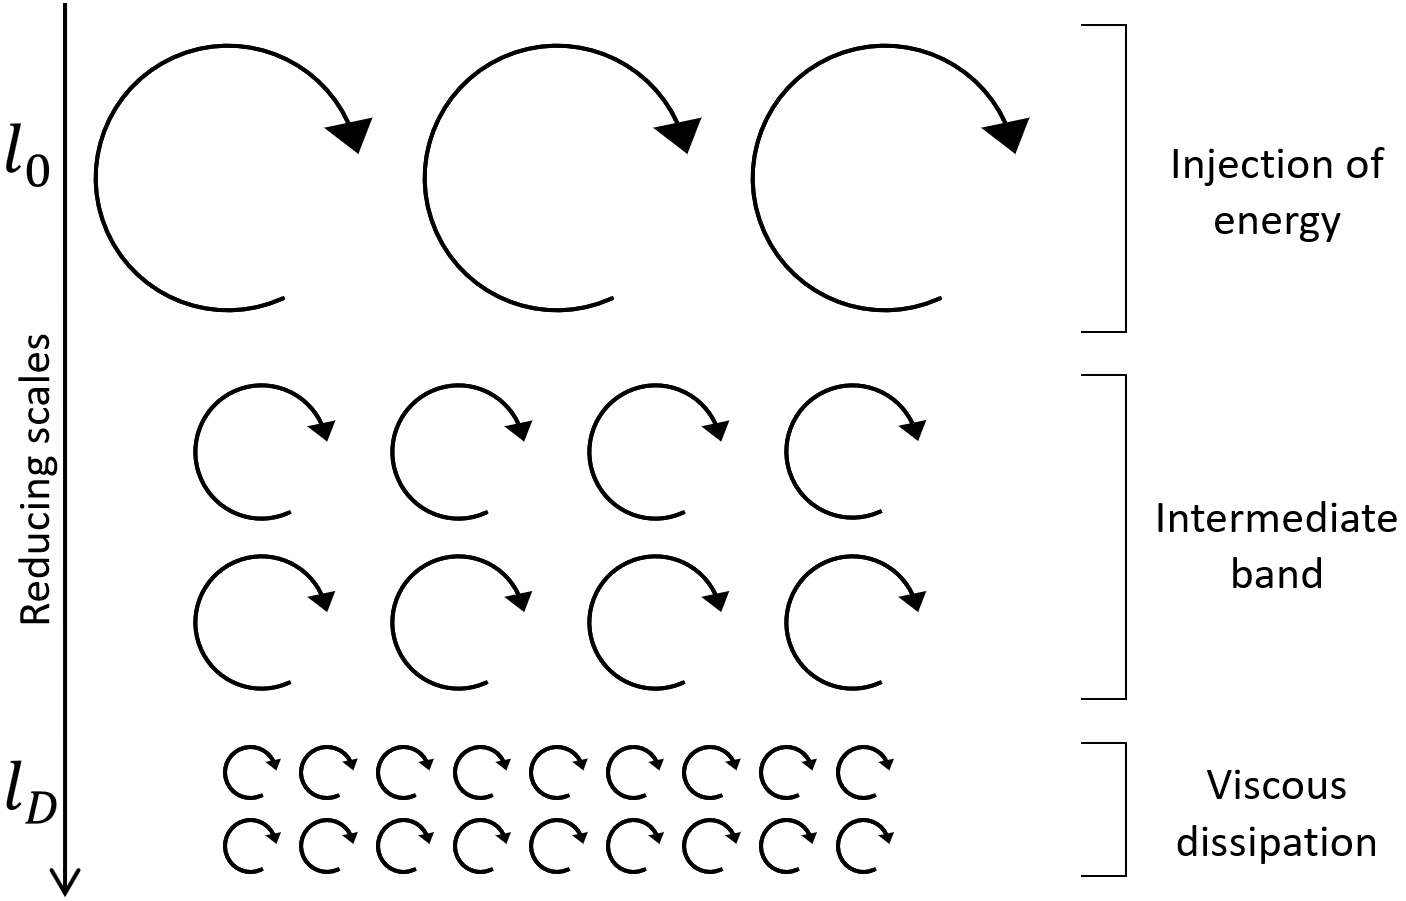
\includegraphics[width=\textwidth]{richardsoncascade.png}
	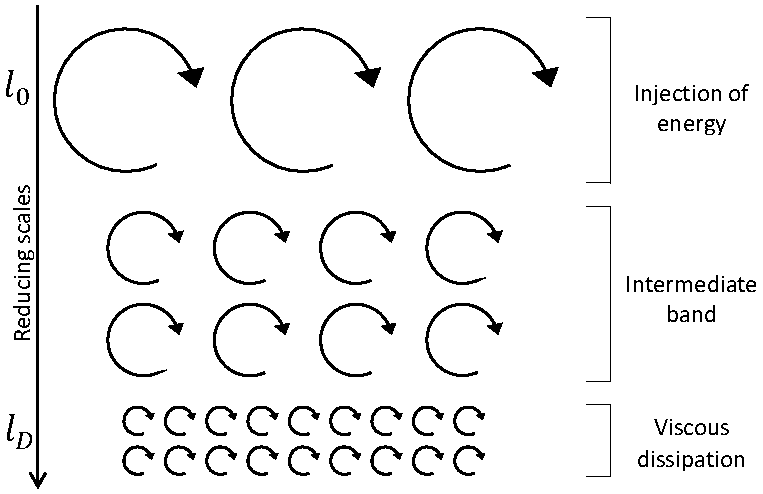
\includegraphics[width=\textwidth]{richardsoncascade.pdf}
	\caption[Richardson energy cascade]{Scheme of the Richardson energy 
	cascade.}
	\label{fig:cascade}
\end{figure}
%

\subsubsection{Simulation of turbulent flows}
From the Kolmogorov theory we can obtain useful information for the simulation 
of turbulent flows. Let us indicate with $l_0$ the length scale at which 
eddies are generated and with $l_D$ the length scale at which they dissipate. 
Then, according to \cite{turbo:kolmogorov}, it can be obtained that
\begin{equation} \label{eq:scaleratio}
	\frac{l_0}{l_D} \sim Re^\frac{3}{4}.
\end{equation}
If we want to perform a reliable simulation of a turbulent flow using the 
Navier-Stokes equations \eqref{eq:nsmass}-\eqref{eq:nsmom}, we need a grid with 
a spatial resolution sufficient to resolve all the eddies until the smallest 
ones, otherwise we would neglect important information about the viscous 
dissipation of these structures. Assuming to have a domain of size comparable 
to $l_0$, then we need a size of the cells of the grid not bigger than $l_D$ and
from \eqref{eq:scaleratio} we deduce that we need at least $Re^\frac{3}{4}$ 
cells in each of the three dimensions of the domain. Because of the fluctuating 
behaviour of turbulence, we always have to perform unsteady simulations, so let 
us denote with $t_0$ the characteristic time of evolution of the eddies at 
$l_0$ and with $t_D$ the characteristic time of evolution of the eddies at 
$l_D$. Again from \cite{turbo:kolmogorov} we have that
\begin{equation}
\frac{t_0}{t_D} \sim Re^\frac{1}{2}.
\end{equation}
The total number of ``operations'' $N$ needed in a simulation can be considered 
proportional to:
\begin{equation}
	N \sim  N_t N_\text{elem},
\end{equation}
where $N_t$ is the total number of time-steps and $N_\text{elem}$ is the total 
number 
of elements in the grid and. From the previous relations we obtain:
\begin{equation}
	N \sim N_t N_\text{elem} \sim \frac{t_0}{t_D} \bigg(\frac{l_0}{l_D}\bigg)^3 
	= Re^\frac{11}{4}.
\end{equation}
%so we need at least $Re^\frac{1}{2}$ time-steps. Globally we end up with a 
%number of 
%degrees of freedom of the order of
%\begin{equation}
%	\# dof \sim \frac{t_0}{t_D} \bigg(\frac{l_0}{l_D}\bigg)^3 = Re^\frac{11}{4}.
%\end{equation}
Reynolds numbers can be easily of the order of $\num{e6}$ or greater in common 
situations, so even with this rough estimate we can see that the computational 
effort for these simulations, called Direct Numerical Simulations (DNS), is 
usually very high. Moreover such a detailed information that we would obtain 
usually goes beyond the real need in many applications, therefore other 
approaches have been developed in order to solve this issue, such as the one 
proposed by the RANS equations.
%
\subsubsection{RANS equations}
The Reynolds Averaged Navier-Stokes (RANS) equations focus on the mean flow 
field, avoiding to simulate all the eddies but without forgetting to take into 
account their effect. In engineering applications this is the most common way 
to simulate turbulent flows because it is cheap and usually the mean 
information is enough for many applications, but we must not forget that 
the obtained result is not the flow field as it appears in reality.
In case that more detail is needed, another approach is given by the Large 
Eddy Simulations (LES), that consist in applying a filter to the Navier-Stokes 
equation that let us resolve the eddies until a certain threshold size.

The first step towards the RANS equations is to decompose each instantaneous 
quantity in the sum of a mean value $\bar{\cdot}$ and a fluctuation $\cdot'$: 
\begin{equation} \label{eq:decomp}
\mathbf{v} = \bar{\mathbf{v}} + \mathbf{v}', \quad p = \bar{p} + p'.
\end{equation}
According to \cite{main:vermal} the mean value can be obtained with a time 
average over a long time interval 
for steady flows, while it is obtained with an ensemble average for unsteady 
flows, so that by definition
\begin{equation}
	\overline{\mathbf{v}'} = \mathbf{0}, \quad \overline{p'}=0.
\end{equation}
We want equations for the mean 
velocity $\bar{\mathbf{v}}$ and the mean pressure $\bar{p}$, so we apply the 
average operation to the Navier-Stokes equations 
\eqref{eq:nsmass}-\eqref{eq:nsmom} and we obtain:
\begin{align}
\label{eq:ransmass} \nabla \cdot \bar{\mathbf{v}} = 0&\\
\label{eq:ransmom} \frac{\partial \bar{\mathbf{v}}}{\partial t} + \nabla \cdot 
( 
\bar{\mathbf{v}} \bar{\mathbf{v}}^\mathrm{T}) + \nabla \cdot 
(\overline{\mathbf{v}' {\mathbf{v}'}^\mathrm{T}})- \nabla \cdot (\nu \nabla 
\bar{\mathbf{v}}) +\frac{1}{\varrho} \nabla \bar{p} - \mathbf{g} = \mathbf{0}&
\end{align}
For what concerns the continuity equation, the average commutes with the 
divergence operator, so we obtain that also the mean velocity has to fulfil the 
incompressibility constraint \eqref{eq:ransmass}. Averaging the momentum 
equation all the terms behave analogously, except the non linear term which 
produces an extra contribution:
\begin{equation}
	\overline{\mathbf{v} \mathbf{v}^\mathrm{T}} = \overline{(\bar{\mathbf{v}} + 
	\mathbf{v}') (\bar{\mathbf{v}} + \mathbf{v}')^\mathrm{T}} = 
	\bar{\mathbf{v}} \bar{\mathbf{v}}^\mathrm{T} + \overline{\mathbf{v}' 
	{\mathbf{v}'}^\mathrm{T}}.
\end{equation}
The new term
\begin{equation}
\tau_R = -\varrho \overline{\mathbf{v}' {\mathbf{v}'}^\mathrm{T}}
\end{equation}
is called Reynolds stress tensor. Mathematically, it expresses the correlation 
between the components of the instantaneous velocity field, while physically it 
represents the diffusive effect of turbulence (see \cite{main:vermal}).
%
\subsubsection{Boundary layers} \label{subsec:bl}
When a fluid flows along a boundary, such as a solid wall, the region near the 
the wall is called boundary layer and it is important because the 
viscosity plays a major role there, even in turbulent conditions.
Independently of the flow regime, the no-slip condition imposes a null velocity 
at the wall and thus a gradient orthogonal to the flow direction. The thickness 
of the boundary layer $\delta$ is conventionally defined as the position where 
the velocity reaches the 99\% of its maximum value and different values are observed for 
different kinds of flow.  See for example \cite{bl:schlichting}, \cite{main:pope} or \cite{main:davidson} for a complete description.

\begin{figure}
	\centering
	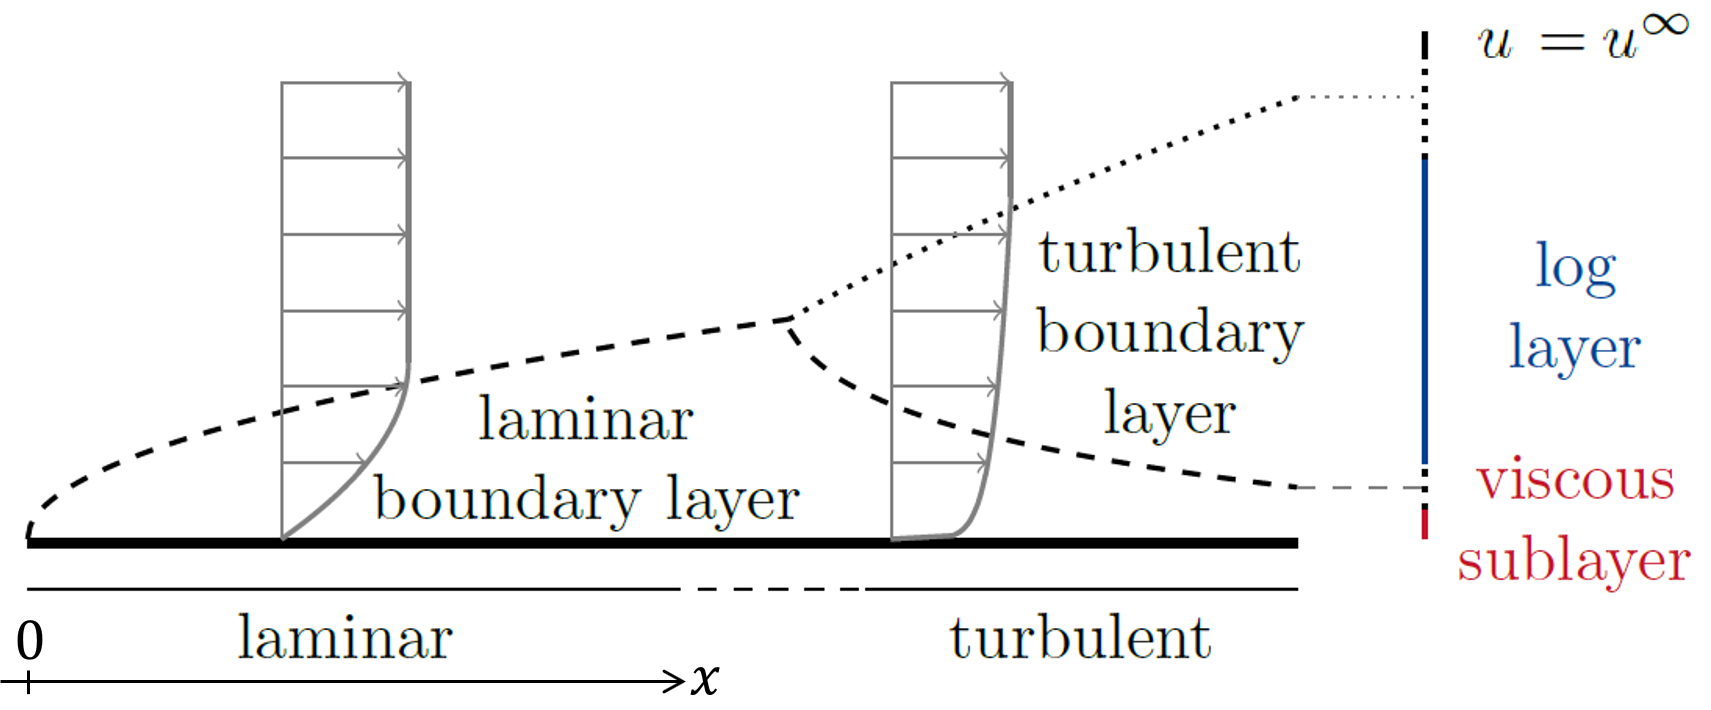
\includegraphics[width=0.8\textwidth]{boundary_layer_axis.png}
	\caption[Boundary layer along a flat plate]{Scheme of the evolution of a 
	boundary layer along a flat plate. The origin of the $x$-axis is set at the stagnation point. Figure source: \cite{tesi:fetzer}.}
	\label{fig:bl}
\end{figure}
Let us consider a flow over a flat plate as depicted in Figure~\ref{fig:bl}: when 
the flow reaches the plate a laminar boundary layer starts to develop. Initially a laminar regime holds and the layer is characterized by a moderate gradient of the 
velocity profile at the wall. After a certain distance a turbulent boundary 
layer starts to grow: it is thicker but the gradient of the velocity at the 
wall is stronger. We can define a Reynolds number based on the distance from 
the beginning of the plate and another one based on the boundary layer 
thickness, respectively
\begin{equation}
Re_x = \frac{u^\infty x}{\nu}, \quad Re_\delta = \frac{u^\infty 
	\delta}{\nu},
\end{equation}
where $u^\infty$ is the maximum velocity far from the wall.

For the laminar boundary layer the profile can be computed analytically 
through the Blasius equation, which is obtained using dimensional arguments (see \cite{bl:schlichting}). 
The thickness grows as the square root $x$, i.e. the distance from the stagnation point:
\begin{equation}
\delta(x) = 4.9 \frac{x}{\sqrt{Re_x}} = 4.91\sqrt{\frac{x 
		\nu}{u^\infty}}.
\end{equation}
When $Re_\delta$ is higher than a certain threshold, the turbulent boundary 
layer begins, but in this case the velocity profile can be expressed only 
through some empirical laws. In order to do that it is useful to define a 
non-dimensional wall coordinate:
\begin{equation}
y^+ = \frac{u_* y}{\nu}, \quad u_* = \sqrt{\frac{\tau_w}{\varrho}},
\end{equation}
where $\tau_w$ is the shear stress at the wall. In the boundary layer four 
different regions can be identified:
\begin{itemize}
	\item near the wall, for approximately $y^+ < 5$, a small laminar viscous 
	sublayer is 
	always present and it cannot be neglected. In this area the viscous 
	stresses are dominant over the Reynolds stresses and the velocity profile 
	can be approximated with a linear relation:
	\begin{equation}
	u = u_* y^+,
	\end{equation}
	\item after that there is a buffer layer in which the viscous and Reynolds 
	stresses are comparable,
	\item then, approximately in the region $30 < y^+ < 150$, there is the so 
	called log-layer, in which the velocity profile can be approximated with a 
	logarithmic function:
	\begin{equation} \label{eq:loglaw}
	u = u_* \bigg( \frac{1}{\kappa} \log y_+ + A\bigg), \quad \kappa=0.41, 
	\quad A = 
	5.5,
	\end{equation}
	where $\kappa$ is the von K\'arm\'an constant,
	\item at last there is an external region, in which the behaviour depends 
	on the external flow field.	
\end{itemize}
Be aware that the numbers given above as bounds for $y^+$ are not universal but 
are very problem-dependent.
\subsubsection{Turbulence models}
The quantity $\tau_R$ is a symmetric tensor with $dim \times dim$ entries, so 
in three 
dimensions we have 6 new unknowns that need to be modelled in order to close 
the problem, this procedure is known as turbulence modelling.
In 1877 \textcite{ipo:boussinesq} suggested that $\tau_R$ could be similar to the viscous 
stress tensor, thus expressed as
\begin{equation} \label{eq:bouss}
\tau_R = 2\mu_t \bar{\mathbf{S}} - 
\frac{2}{3}\varrho k \mathbb{1}.
\end{equation}
The first term has the same form of $\tau$ if we consider the mean velocity 
field, 
the only difference is that the dynamic viscosity $\mu$ is substituted by a 
turbulent viscosity $\mu_t$ [$\si{\pascal \second}$]. The second term is needed 
to model the isotropic part of $\tau_R$ correctly:
\begin{equation} \label{eq:tracciatau}
tr(\tau_R) = -tr(\varrho \overline{\mathbf{v}' {\mathbf{v}'}^\mathrm{T}}) = 
-\varrho \sum_{i=1}^{dim} \overline{(v_i')^2} = -2\varrho k,
\end{equation}
where $k$ is the turbulent kinetic energy defined as
\begin{equation}
k = \frac{1}{2} \sum_{i=1}^{dim} \overline{(v_i')^2},
\end{equation}
while exploiting equation \eqref{eq:ransmass} we get
\begin{equation}
	tr(2\mu_t \bar{S}) = 2 \mu_t \sum_{i=1}^{dim} \frac{\partial 
	\bar{v}_i}{\partial x_i} = 2\mu_t (\nabla \cdot \bar{\mathbf{v}}) = 0.
\end{equation}
With this hypothesis $\mu_t$ and $k$ are the only unknowns left and the 
momentum equation \eqref{eq:ransmom} becomes:
\begin{equation} \label{eq:ransmom2}
\frac{\partial \bar{\mathbf{v}}}{\partial t} + \nabla 
\cdot ( \bar{\mathbf{v}} \bar{\mathbf{v}}^\mathrm{T}) - \nabla \cdot 
(\nu_\text{eff} \nabla \bar{\mathbf{v}}) + \frac{1}{\varrho}\nabla (\bar{p} + 
\frac{2}{3}\varrho k) - \mathbf{g} = \mathbf{0},
\end{equation}
where we have introduced an effective kinematic viscosity
\begin{equation}
	\nu_\text{eff} = \nu + \nu_t, \quad \nu_t = \frac{\mu_t}{\varrho}.
\end{equation}
Since for incompressible fluids we have removed the thermodynamic relation 
between $\varrho$ and $p$, we can consider as unknown a generalized pressure 
$p_\text{gen}$ such that:
\begin{equation}
p_\text{gen} = \bar{p} + \frac{2}{3}\varrho k,
\end{equation}
reducing the unknowns to $\nu_t$ alone, which can be estimated using different 
turbulence models.

The idea of the Boussinesq hypothesis \eqref{eq:bouss} comes partially from an 
analogy 
between the motion 
of the turbulent structures and the molecular motion, but there are cases in 
which it can be shown that this hypothesis leads to poor results (see 
\cite{main:pope}). There exist also turbulence models called Reynolds stress 
equations models (RSM) that do not use it and try to find equations for 
all the entries of the Reynolds stress tensor, but in this way a large set of 
equations is obtained and consequently the required computational effort 
increases. See \cite{main:pope} or \cite{main:vermal} for more information.

From now, on the over-bar used to denote averaged quantities will be 
neglected in order to simplify the notation.

\subsubsection{Zero-equations models}
The simplest turbulence models are called zero-equations models or algebraic 
models because they compute the turbulent viscosity using an algebraic relation 
that exploits geometrical quantities, so they do not introduce any additional 
PDE to the problem. Due to their simplicity they were used in the past years 
when the computational resources were limited, but they have intrinsic weak 
points and they can be applied only in special simple situations.

An important example is Prandtl's \emph{mixing length} model \cite{turbo:prandtl}. It is 
useful with two-dimensional flows when the mean velocity field has a dominant 
direction and the gradient in the longitudinal direction is negligible with 
respect to that in the orthogonal direction. Let us assume that $u$ is the 
main component of the velocity and that the flow is bounded by a wall at $y=0$. 
From dimensional considerations it can be assumed that
\begin{equation}
\nu_t = l_\text{mix}v_\text{mix},
\end{equation}
where $l_\text{mix}$ and $v_\text{mix}$ are a characteristic length scale and a 
velocity 
scale of turbulence. Then, it is reasonable to choose
\begin{equation}
	v_\text{mix} = l_\text{mix} \left\lvert \frac{\partial u}{\partial y} 
	\right\rvert,
\end{equation}
because the shear stress in the mean flow gives its contribution to the 
turbulent mixing of the largest eddies. At last, $l_\text{mix}$ is chosen from 
empirical considerations derived from the boundary layer theory previously 
described. For example,
\begin{equation}
l_\text{mix} = \kappa y,
\end{equation}
in the original version, or
\begin{equation}
l_\text{mix} = \kappa y[1 - exp(y^+ / 26)],
\end{equation}
using a correction proposed by \textcite{turbo:vandriest} that dampens $\nu_t$ for $y \rightarrow 0$.
%
\subsubsection{$k\text{-}\varepsilon$ model}
Two-equation models involve the solution of two additional PDEs and the 
$k\text{-}\varepsilon$ is probably the most famous one in this category. The 
key contribution to this model was given by \textcite{turbo:ke}. It is 
based on the assumption that the turbulent viscosity $\nu_t$ could be correctly 
determined through the turbulent kinetic energy $k$ and its dissipation rate 
$\varepsilon$. Considering the dimension units, the relation must be
\begin{equation}
\nu_t = C_\mu \frac{k^2}{\varepsilon},
\end{equation}
where $C_\mu$ is a non-dimensional constant and $\varepsilon$ is defined as
\begin{equation}
\varepsilon = 2 \nu \overline{\mathbf{S}' \cdot \mathbf{S}'}, \quad \mathbf{S}' 
= \frac{\nabla \mathbf{v}' + (\nabla \mathbf{v}')^\mathrm{T}}{2}.
\end{equation}

Starting from the momentum equation of the Navier-Stokes model \eqref{eq:nsmom} 
and from the decomposition in mean value plus fluctuation \eqref{eq:decomp}, we 
derive an equation for $k$:
\begin{equation}
	\frac{\partial k}{\partial t} + \nabla \cdot (k\mathbf{v}) - \nabla \cdot
	\bigg[ \bigg(\nu + \frac{\nu_t}{\sigma_k}\bigg) \nabla k\bigg] 
	-2\nu_t \mathbf{S} \cdot \mathbf{S} + \varepsilon = 0,
\end{equation}
where $\sigma_k$ is a non-dimensional constant. In a similar way we could 
derive an evolution equation for $\varepsilon$, but it would contain too many 
terms difficult to model and to measure, so an empirical equation built in 
analogy with the one for $k$ is used instead:
\begin{equation} \label{eq:epsilon}
		\frac{\partial \varepsilon}{\partial t} + \nabla \cdot (\varepsilon 
		\mathbf{v}) - \nabla \cdot \bigg[ \bigg(\nu + 
		\frac{\nu_t}{\sigma_\varepsilon} 
		\bigg) \nabla \varepsilon \bigg] - C_{\varepsilon_1} 
		\frac{\varepsilon}{k} 2 \nu_t \mathbf{S} \cdot \mathbf{S} + 
		C_{\varepsilon_2}\frac{\varepsilon^2}{k} = 0.
\end{equation}
The standard model sets the following constants (see \cite{main:vermal}):
\begin{equation}
	C_\mu = 0.09, \quad \sigma_k = 1, \quad \sigma_\varepsilon = 1.3, \quad 
	C_{\varepsilon_1} = 1.44, \quad C_{\varepsilon_2} = 1.92.
\end{equation}

This model behaves best for confined flows and high Reynolds number, where 
the Reynolds stresses are dominant. Near the wall this assumption fails, so it 
is common to use a wall function such as the one given by the boundary layer 
theory \eqref{eq:loglaw} in order to compute the velocities at the cells near 
the wall. This can be done easily for flat walls and it brings also 
computational advantages, because we can avoid to have very small cells near 
the wall to resolve the viscous sublayer.

Over the years, many variants of this model have been developed, for example 
the \emph{RNG}~$k\text{-}\varepsilon$ model, which is derived with a different 
procedure with the purpose of improving the equation for
$\varepsilon$, or the \emph{low-$Re$}~$k\text{-}\varepsilon$ model, which 
adds extra terms in order to correctly model the behaviour near the wall. See 
\cite{main:vermal} for more details.
%
\subsubsection{$k\text{-}\omega$ model}
The $k\text{-}\omega$ model is another two-equations model that uses a specific 
dissipation rate $\omega$ instead of the dissipation rate $\varepsilon$. It was 
originally proposed by \textcite{komega:kolmo} and subsequently refined many 
times by \textcite{turbo:komega}.

The equation for the turbulent kinetic energy is analogous to the one used in 
the $k\text{-}\varepsilon$ model:
\begin{equation} \label{eq:komegak}
	\frac{\partial k}{\partial t} + \nabla \cdot (k\mathbf{v}) - \nabla \cdot 
\bigg[\bigg(\nu + \sigma^*\frac{k}{\omega}\bigg) \nabla k\bigg] -P + \beta^* k 
\omega = 0,
\end{equation}
with the production term $P$ that can be limited in the following way:
\begin{equation}
	P = \min \{ 2 \nu_t \mathbf{S} \cdot \mathbf{S}, 20 \beta^* k \omega \}.
\end{equation}
The equation for $\omega$ is empirical and driven by physical considerations as 
it was the equation \eqref{eq:epsilon} for $\varepsilon$. It reads:
\begin{equation} \label{eq:komegaomega}
	\frac{\partial \omega}{\partial t} + \nabla \cdot (\omega \mathbf{v}) - 
	\nabla \cdot \bigg[ \bigg( \nu + \sigma \frac{k}{\omega} \bigg) \nabla 
	\omega 
	\bigg] - \alpha \frac{\omega}{k} 2 \nu_t \mathbf{S} \cdot \mathbf{S} 
	-\frac{\sigma_d}{\omega} \nabla k \cdot 
	\nabla \omega+ \beta \omega^2 = 0.
\end{equation}
The term
\begin{equation}
\frac{\sigma_d}{\omega} \nabla k \cdot \nabla \omega
\end{equation}
is a new addition with respect to \eqref{eq:epsilon}. It is related to cross-diffusion and its activation depends on the 
direction of the gradients of $k$ and $\omega$:
\begin{equation}
\sigma_d =
\begin{cases}
0 &\text{if $\nabla k \cdot \nabla \omega \leq 0$}\\
\sigma_{do} &\text{if $\nabla k \cdot \nabla \omega > 0$}
\end{cases},
\quad \sigma_{do} = \frac{1}{8}.
\end{equation}
The turbulent viscosity $\nu_t$ is obtained as
\begin{equation}
\nu_t = \frac{k}{\tilde{\omega}}, \quad \tilde{\omega} = \max \Bigg\{ \omega, 
C_\text{lim} \sqrt{ 2\frac{\mathbf{S}\cdot\mathbf{S}}{\beta^*}} \Bigg\}.
\end{equation}
The model is closed with the following empirical coefficients:
\begin{equation}
	\beta^* = \frac{9}{100}, \quad \sigma^* = \frac{3}{5}, \quad \alpha = 
	\frac{13}{25}, \quad \beta = \frac{177}{2500}, \quad \sigma = \frac{1}{2}, 
	\quad C_\text{lim} = \frac{7}{8}.
\end{equation}

The interpretation of $\omega$ is not straight-forward: originally it was 
defined by Kolmogorov as ``the rate of dissipation of energy in unit volume and 
time'', therefore defined as
\begin{equation}
	\omega = \frac{k}{\varepsilon}.
\end{equation}
Other contributors to the development of this model have referred to it as 
the the root mean square (RMS) of the fluctuating vorticity, i.e.
\begin{equation}
	\omega = \sqrt{\overline{ (\boldsymbol\omega ')^2 }}, \quad 
	\boldsymbol\omega = \nabla \times \mathbf{v}.
\end{equation}
In this case, $\omega^2$ is the double of the \emph{enstrophy}, which is a 
quantity associated to the energy related to vorticity.

This model has shown good results also near boundaries, so it does not 
require any wall correction. For our purposes it is the most appropriate choice 
because we would like to have non-flat boundaries, so employing a 
wall law would be cumbersome, if not impossible. Moreover, the values near the boundary are 
very important in our tests, because they influence the exchange processes 
across the interface between free-flow and porous-medium flow.

As boundary conditions, we have:
\begin{itemize}
	\item on inflow boundaries, Dirichlet conditions are set both for $k$ and 
	$\omega$. According to \cite{ko:ansys}, the following formulas can be used:
	\begin{equation} \label{eq:koic}
		k = \frac{3}{2} (|\!|\mathbf{v}_\text{in}|\!|	 I)^2, \quad \omega = 		
		\frac{100k^{1/2}}{7C_\mu^{1/4}L},
	\end{equation}
	where $\mathbf{v}_\text{in}$ is the inflow velocity and $I$ is a 
	non-dimensional quantity called turbulence intensity that could be 
	estimated as
	\begin{equation}
	I = \frac{0.16}{Re^{1/8}}.
	\end{equation}
	Here, $C_\mu=0.09$ and $L$ is a characteristic size of the domain,
	\item on solid walls, $k=0$, while, according to 
	\cite{main:wilcox}, the following asymptotic behaviour for $\omega$ is used:
	\begin{equation}
		\omega \rightarrow \frac{6 \nu}{\beta d^2} \quad \text{as} \quad d 
		\rightarrow 0,
	\end{equation}
	where $d$ is the distance from the nearest wall,
	\item on outflow and symmetry boundaries, a zero-gradient condition is 
	assumed:
	\begin{equation}
		\nabla k \cdot \mathbf{n} = 0, \quad \nabla \omega \cdot \mathbf{n} = 0.
	\end{equation}
\end{itemize}
%
\section{Porous-medium flow} \label{sec:pm}
According to \cite{forch:nield} a porous-medium is ``a material consisting of a 
solid matrix with an interconnected void''. The void spaces are called 
\emph{pores} and they allow a fluid to flow through the material. We consider the 
solid matrix to be fixed, neglecting the fluid-structure interaction. Examples 
of porous-media are sand, wood, soil, 
sandstone and ceramics.

To simulate flow through a porous medium theoretically we could use 
the standard fluid dynamics equations at the pore scale, but this approach is
extremely expensive because of the strict spatial and temporal requirement of a direct numerical simulation in such a complex domain. Moreover, from the point of view of applications, the knowledge of the model variables at such level of detail is often useless, considering also the fact that at this scale they are very irregular and, also, it is hard to get measurements of them.
What is usually done is to 
upscale the description of the flow by considering averaged quantities within a 
Representative Elementary volume (REV), thus considering the 
porous-medium as a continuum at a larger scale. In this way we lose the 
information at the pore scale, but we obtain results that 
are comparable to experimental measurements. The upscaling procedure can be done by rigorous homogenization techniques \cite{homo:allaire} or by formal averaging \cite{volaver:withakerbook}. We briefly describe the latter approach.

Given a domain $\Omega_\text{pm}$ occupied by the porous-medium, we consider 
at every point $\mathbf{x} \in \Omega_\text{pm}$ a ball $B_r(\mathbf{x})$ of 
radius $r$, that will be the REV. Starting from a function $f$ defined at the 
pore scale we compute its average $\hat{f}$:
\begin{equation}
	\hat{f}(\mathbf{x}) = \frac{1}{|B_r(\mathbf{x})|} \int_{B_r(\mathbf{x})} 
	f(\mathbf{y}) d\mathbf{y}, \quad \forall \mathbf{x} \in \Omega_\text{pm}.
\end{equation}
The radius $r$, and thus the dimension of the REVs, should be chosen such that
\begin{equation}
	l \ll r \ll L,
\end{equation}
where $l$ is the pore scale size and $L$ is the macro scale size, as for 
example in Figure~\ref{fig:rev}. In such a way 
the high frequency variations of microscopic properties are averaged out at the REV scale, but the low frequency variations of macroscopic properties are kept (see \cite{main:helmig}).
\begin{figure}
	\centering
	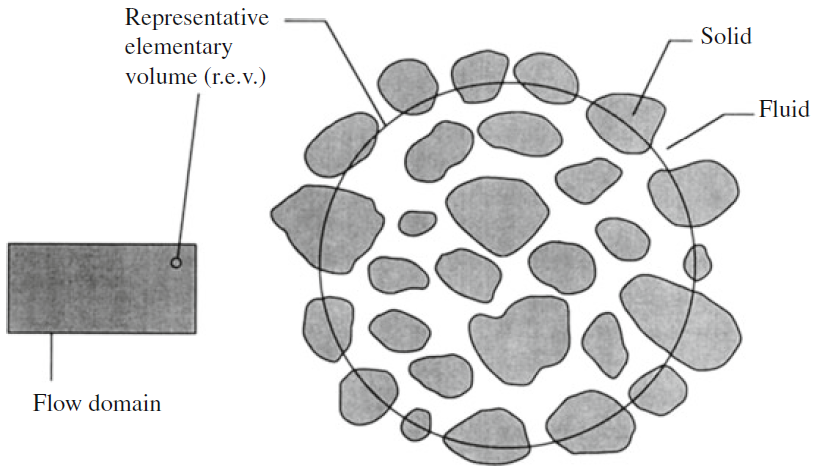
\includegraphics[width=\textwidth]{rev.png}
	\caption[REV in a porous-medium]{An example of a REV in a porous-medium. 
	Comparison of its size with the one of the pores and the one of 
	$\Omega_\text{pm}$. Figure source: \cite{forch:nield}.}
	\label{fig:rev}
\end{figure}

Let us define the \emph{porosity} of the porous-medium as
\begin{equation}
\varphi(\mathbf{x}) = \frac{1}{|B_r(\mathbf{x})|} \int_{B_r(\mathbf{x})} \chi 
(\mathbf{y}) d\mathbf{y},
\end{equation}
where $\chi(\mathbf{x})$ is the characteristic function of the void space:
\begin{equation}
\chi(\mathbf{x}) =
\begin{cases}
1 &\text{if $\mathbf{x}$ is void}\\
0 &\text{if $\mathbf{x}$ is not void}
\end{cases}, \quad \forall \mathbf{x} \in \Omega_\text{pm}.
\end{equation}

For simplicity we will assume to have porous-media with constant porosity. In 
natural materials usually $\varphi$ is not greater then $0.6$, but for some 
artificial materials, such as metallic foams, $\varphi$ could be almost $1$.
We will also consider only single-phase, single-component flows.
%
\subsection{Continuity equation}
The governing equations for a porous-medium at the REV scale can be computed 
from the standard equations for the fluid through the application of volume 
averaging techniques (see \cite{volaver:withakerbook}).

We obtain the following continuity equation:
\begin{equation}
\varphi\frac{\partial \varrho}{\partial t} + \nabla \cdot (\varrho 
\mathbf{v}) = 0,
\end{equation}
where $\varrho$ denotes the density of the fluid. $\mathbf{v}$ is the velocity 
obtained averaging over a REV containing both fluid and solid and it can be 
called \emph{Darcy} velocity or \emph{seepage} velocity. It should not be 
confused with the \emph{intrinsic} velocity $\mathbf{V}$ that we would obtain 
averaging over a REV containing only fluid, as they are related by:
\begin{equation}
	\mathbf{v} = \varphi \mathbf{V}.
\end{equation}

If we assume that the fluid is incompressible, then the continuity equation 
reduces to
\begin{equation} \label{eq:pmcontinuity}
\nabla \cdot \mathbf{v} = 0.
\end{equation}
%
\subsection{Momentum equation}
According to the assumptions, we can obtain different laws.
\subsubsection{Darcy's law}
For the momentum equation the most common choice is the Darcy's law:
\begin{equation} \label{eq:darcy}
	\mathbf{v} = -\frac{1}{\mu}\mathbf{K} (\nabla p - \varrho \mathbf{g}),
\end{equation}
where $\mathbf{K}$ [$\si{m^2}$] is the permeability tensor of the 
porous-medium; it is symmetric and positive-definite and it can be simplified 
to a scalar for isotropic porous-media. 
This equation holds for creeping flows, with $Re < 1$, for which 
inertial effect can be neglected.

It was first obtained experimentally by Henry Darcy in 1856, who discovered a 
proportionality between the flow rate and the pressure drop across a uniform 
porous-medium. After that there have been many attempts to derive it analytically, 
starting from the Navier-Stokes equations and using volume averaging techniques 
with different assumptions made, see for example \cite{volaver:ithakerdarcy}. 
Moreover it can be obtained through a homogenization procedure if the 
porous-medium is periodic (see \cite{homo:holmes}).

The permeability is a quantity that depends only on the geometry of the porous 
medium and not on the flow, typical values range from $\SI{e-7}{m^2}$ of 
gravel to $\SI{e-16}{m^2}$ of limestone.
There are models to compute it in the case of simple geometries, for example 
through the Carman-Kozeny equation (see \cite{forch:nield}). 
%
\subsubsection{Forchheimer's law}
There exist many generalizations of Darcy's law, for example to multiphase 
and multicomponent flows, to non-Newtonian fluids or, as in this case, to 
higher Reynolds numbers. The 
extension that we are interested in is the so called Forchheimer's law \cite{forch:1901}, that reads:
\begin{equation} \label{eq:forch}
	\mathbf{v} + C_F \sqrt{\mathbf{K}} \frac{\varrho}{\mu} 
	|\mathbf{v}|\mathbf{v} = - \frac{1}{\mu} \mathbf{K}(\nabla p - \varrho 
	\mathbf{g} ),
\end{equation}
where the second term is added to the Darcy's law in order to take into account any possible inertial effect. $C_F$ is a non-dimensional coefficient which is 
here taken equal to $0.55$, even if there exist many different corrections (see 
\cite{forch:nield} and \cite{forch:tesi}).

As reported by \textcite{forch:nield}, the equation was originally proposed by 
Forchheimer in 1901, but the dependence on $\sqrt{\mathbf{K}}$ was later introduced 
by \textcite{forch:ward}. \textcite{volaver:withakerforch} 
derived it with the volume averaging  starting from the Navier-Stokes equations.

This equation holds when the flow in the porous-medium is laminar, but 
the drag from linear becomes quadratic because the contribution due to solid 
obstacles becomes comparable to the one due to friction. According to 
\cite{forch:nield}, the transition from a linear to a quadratic regime is 
smooth and takes place at
\begin{equation}
	Re_\mathrm{K} \simeq 100,
\end{equation}
where $Re_\mathrm{K}$ is a Reynolds number based on the square root of the 
permeability:
\begin{equation}
	Re_\mathrm{K} = \frac{U \sqrt{\mathrm{K}}}{\nu}.
\end{equation}
%
\section{Coupling conditions} \label{sec:coupling}
At the interface between the free-flow region and the porous-medium we have to 
impose suitable conditions in order to couple the two subdomains. Let us denote 
with $\Omega_\text{ff}$ the free-flow domain and with $\Omega_\text{pm}$ the 
porous-medium domain, then
\begin{equation}
	 \Gamma_\text{int} = \overline{\Omega}_\text{ff} \cap 
	 \overline{\Omega}_\text{pm}
\end{equation}
is the interface between them.

Following \textcite{paper:mosthaf}, we would like to have conditions such that 
the interface could be as close as possible to local thermodynamic 
equilibrium. However, this cannot be rigorously achieved due to the 
different model concepts in the two subdomains. Since we are dealing with 
single-phase, single-component isothermal flows, we only have to impose the 
mechanical equilibrium, for which we need:
\begin{itemize}
	\item the continuity of normal mass fluxes, that in our incompressible case 
	reduces to the continuity of the normal component of the velocity:
	\begin{equation} \label{eq:contmass}
		[\mathbf{v} \cdot \mathbf{n}]_\text{ff} = - [\mathbf{v} 
		\cdot \mathbf{n}]_\text{pm} \quad \text{on $\Gamma_\text{int}$},
	\end{equation}
	where the subscripts $_\text{ff}$ and $_\text{pm}$ denote that the 
	quantities are 
	evaluated in the free-flow or in the porous-medium subdomain. Notice that
	\begin{equation}
		\mathbf{n}_\text{ff} = -\mathbf{n}_\text{pm} \quad \text{on 
		$\Gamma_\text{int}$},
	\end{equation}
	\item the continuity of normal stresses:
	\begin{equation} \label{eq:coupnormalstress}
		[(\varrho \mathbf{v} \mathbf{v}^\mathrm{T} - \mu_\text{eff} \nabla 
		\mathbf{v} + p\mathbb{1}) 
		\mathbf{n}]_\text{ff} = 
		- [p\mathbf{n}]_\text{pm} \quad \text{on $\Gamma_\text{int}$},
	\end{equation}
	that may result in a jump of the pressure at the interface, although pressure is typically a continuous thermodynamic variable,
	\item a condition for the tangential component of the velocity in the 
	free-flow and in particular we use the one proposed by \textcite{inter:bj}:
	\begin{equation}
		\bigg[ \bigg( -\frac{\sqrt{\mathrm{K}}}{\alpha_{BJ}} (\nabla \mathbf{v}) 
		\mathbf{n} - \mathbf{v} \bigg) \cdot \mathbf{t}_i \bigg]_\text{ff} = 
		[\mathbf{v} \cdot \mathbf{t}_i]_\text{pm}, \quad \forall i \in \{1, 
		\dots, dim - 1\},
	\end{equation}
	on $\Gamma_\text{int}$, where $\alpha_\text{BJ}$ is a non-dimensional 
	coefficient that depends on 
	properties of the permeable material and $\mathbf{t}_i, \; 
	i \in \{1, \dots, dim-1\}$ is a basis of the plane tangential to the 
	interface $\Gamma_\text{int}$. With this condition we allow a slip of the 
	tangential component of the velocity and the more the porous-medium is 
	permeable, the more slip is allowed.
	
	We also employ the simplification introduced by \textcite{inter:bjs}:
	\begin{equation}
		[\mathbf{v} \cdot \mathbf{t}_i]_\text{pm} \simeq 0, \quad \forall i \in 
		\{1, 
		\dots, dim-1\},
	\end{equation}
	so we neglect the tangential velocity in the porous-medium since it is very small with 
	respect to the one in the free-flow region, thus obtaining the 
	Beavers-Joseph-Saffman (BJS) condition:
	\begin{equation} \label{eq:bjs}
		\bigg[ \bigg( -\frac{\sqrt{\mathrm{K}}}{\alpha_\text{BJ}} (\nabla \mathbf{v}) 
		\mathbf{n} - \mathbf{v} \bigg) \cdot \mathbf{t}_i \bigg]_\text{ff} = 0, 
		\quad \forall i \in \{1, \dots, dim - 1\}.
	\end{equation}
	This condition can be derived also using homogenizations techniques (see \cite{bjs:homo} and \cite{intro:disca2009}).
\end{itemize} 